\documentclass[english,aspectratio=43]{beamer}

\usetheme{Dresden}

\usepackage{babel}
\usepackage{graphicx}

\beamertemplatenavigationsymbolsempty

\graphicspath{{img/}}

\title{Parameter-based Island Terrain Generation}

\subtitle{Visual Computing Project}

\author[van Dalen, van Dueren den Hollander]{
	Tim van Dalen (0744839)\\
	\and
	Carl van Dueren den Hollander (0742635)
}

\institute[TU/e]
{
    WIS\\
	Eindhoven University of Technology
}

\date{\today}


\subject{Visual Computing Project}

\AtBeginSection[]
{
  \begin{frame}
    \frametitle{Outline}
    \tableofcontents[currentsection]
  \end{frame}
}

\begin{document}

	\begin{frame}
		\titlepage
	\end{frame}

	\begin{frame}
		\frametitle{Outline}
		\tableofcontents
	\end{frame}

	\section{Intro}
	\begin{frame}{Intro}
		\begin{itemize}
			\item Terrain generation
			\item Islands
			\item Biomes
		\end{itemize}
	\end{frame}

	\section{Goal}
	\begin{frame}{Goal}
		\begin{columns}[T]
			\begin{column}{.5\textwidth}
				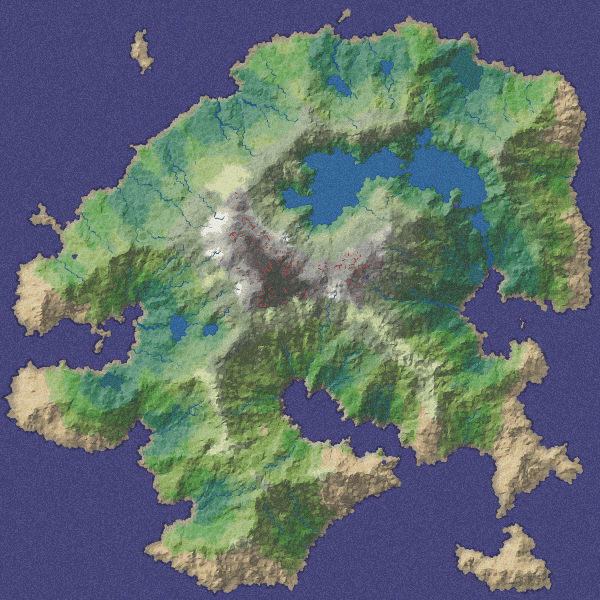
\includegraphics[width=\linewidth]{goal}
			\end{column}
			\begin{column}{.5\textwidth}
				\begin{itemize}
					\item Implement algorithm by Patel
					\item Adjust goals
					\item Flexible generation
					\item Full 3D interactive viewer
				\end{itemize}
			\end{column}
		\end{columns}
	\end{frame}

	\section{Approach}
	\begin{frame}{Approach}
		\begin{itemize}
			\item Separate generator and viewer
			\item Cross-platform
			\item C++
		\end{itemize}
	\end{frame}

	\begin{frame}{Cross platform}
		\begin{itemize}
			\item<1,4-> wxWidgets for GUI
			\item<1-> Two graphics implementations
				\begin{itemize}
					\item Shaders
					\item Old style OpenGL pipeline (mesa compatible)
				\end{itemize}
			\only<1,4->{\item Two goal/test environments
				\begin{itemize}
					\item msvc
					\item gcc
				\end{itemize}}
		\end{itemize}
		\only<2>{
			\centering
			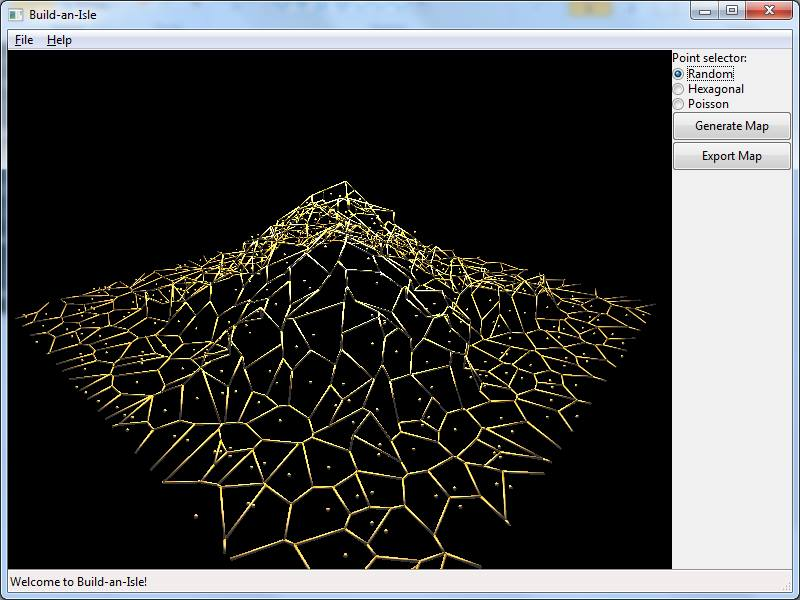
\includegraphics[width=0.5\linewidth]{shader}
		}
		\only<3>{
			\centering
			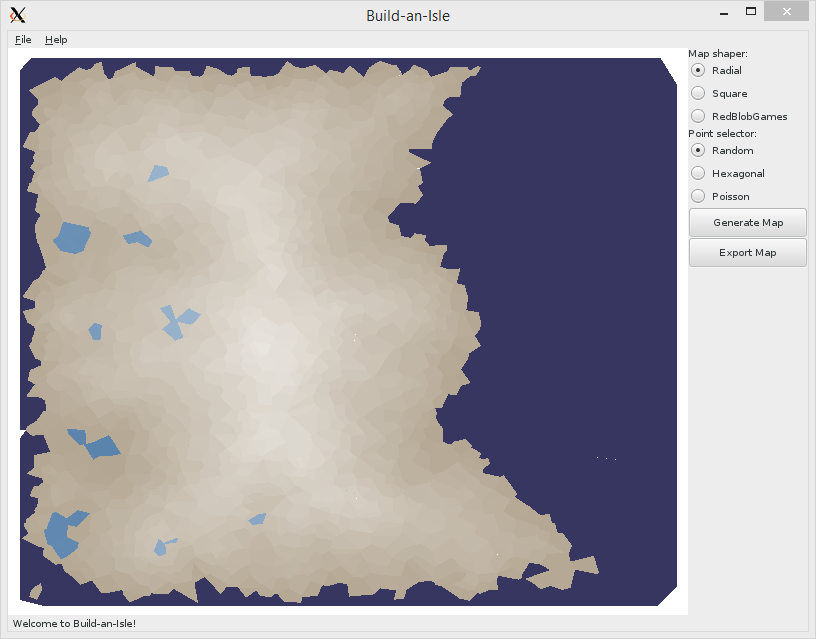
\includegraphics[width=0.5\linewidth]{simple}
		}
	\end{frame}

	\section{Algorithm}
	\subsection{Points}
	\begin{frame}{Point selection}
		\centering
		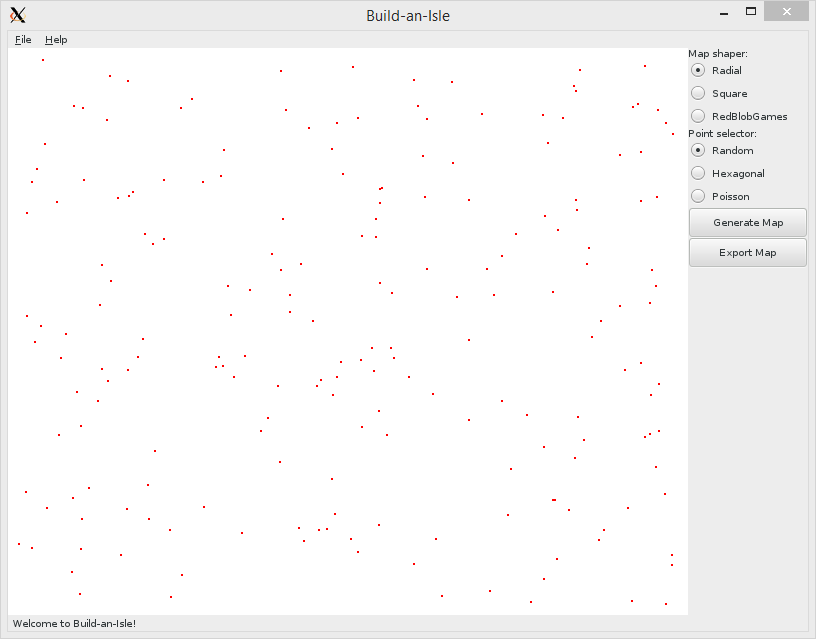
\includegraphics[width=0.7\linewidth]{points}
	\end{frame}

	\subsection{Voronoi}
	\begin{frame}{Calculate Voronoi diagram}
		\centering
		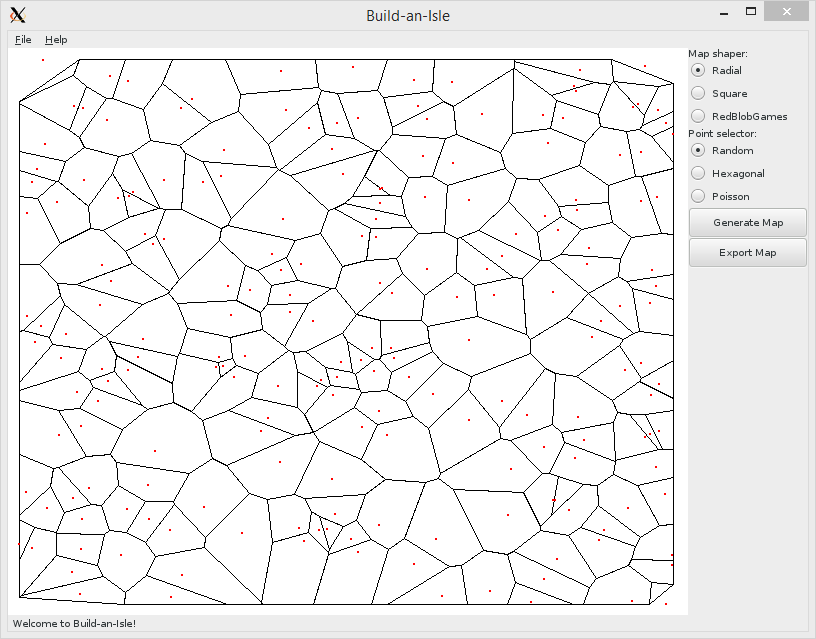
\includegraphics[width=0.7\linewidth]{voronoi}
	\end{frame}

	\subsection{Delaunay}
	\begin{frame}{Calculate Delaunay triangulation}
		\centering
		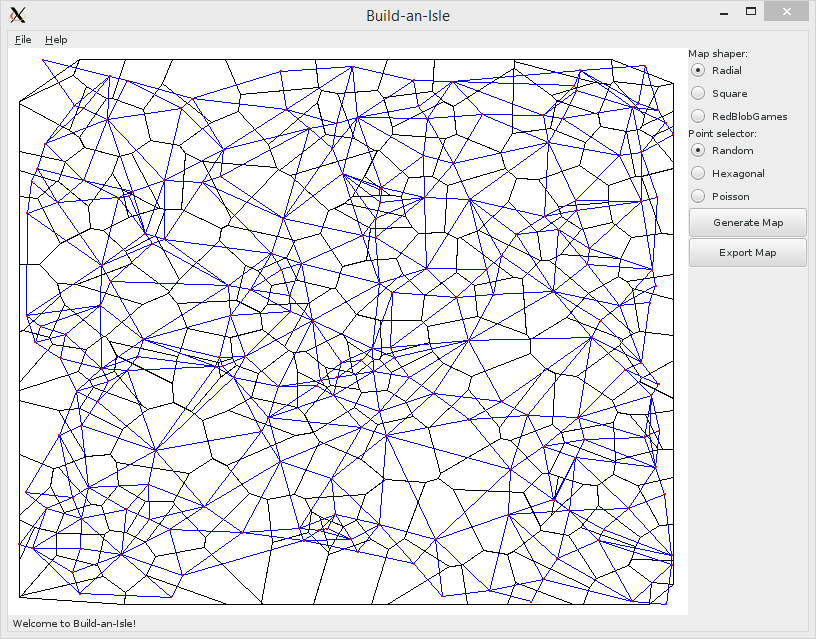
\includegraphics[width=0.7\linewidth]{delaunay}
	\end{frame}

	\subsection{Polygons}
	\begin{frame}{Shape island}
		\centering
		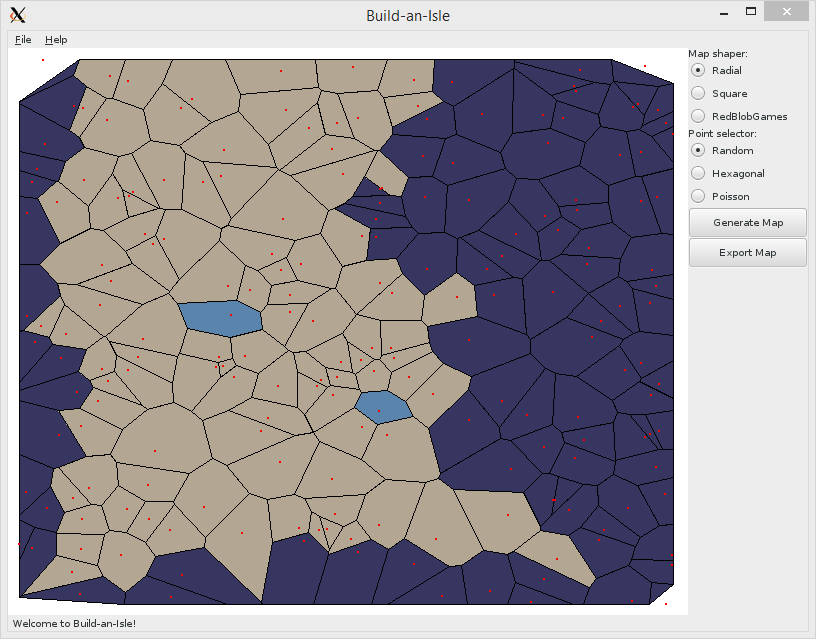
\includegraphics[width=0.7\linewidth]{polygons}
	\end{frame}

	\subsection{Elevation}
	\begin{frame}{Determine elevation}
		\centering
		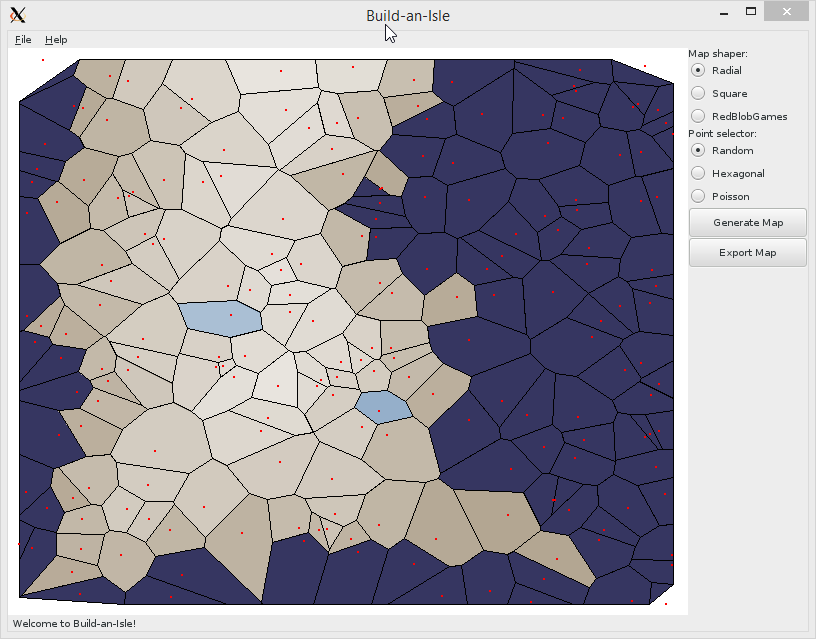
\includegraphics[width=0.7\linewidth]{elevation}
	\end{frame}

	\section{Generator}
	\subsection{Point selection}
	\begin{frame}{Random}
		\centering
		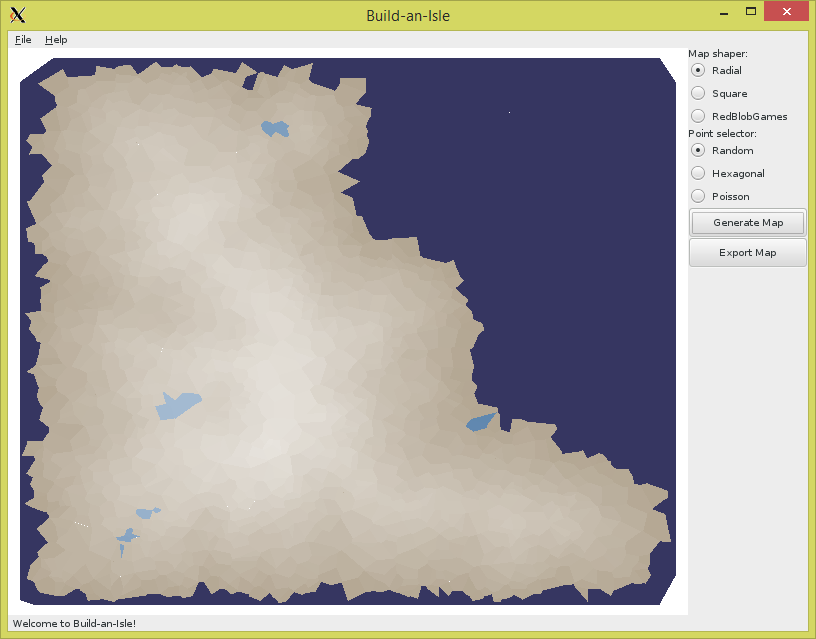
\includegraphics[width=0.7\linewidth]{random}
	\end{frame}

	\begin{frame}{Poisson}
		\centering
		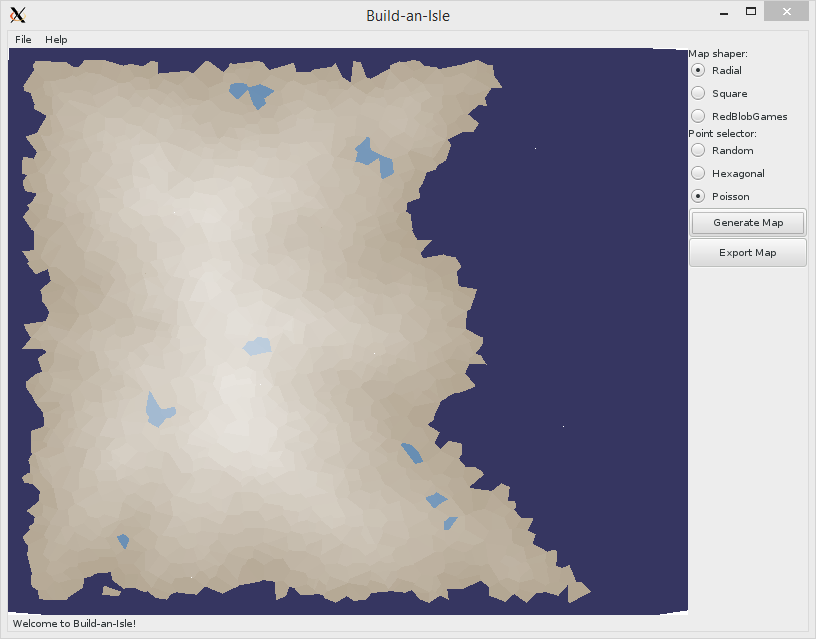
\includegraphics[width=0.7\linewidth]{poisson}
	\end{frame}

	\begin{frame}{Hexagonal}
		\centering
		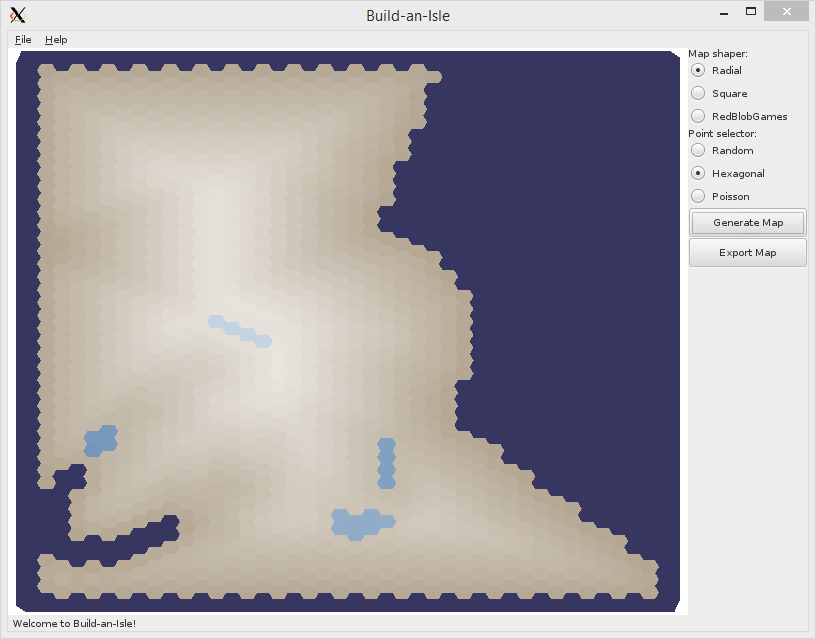
\includegraphics[width=0.7\linewidth]{hex}
	\end{frame}

	\subsection{Map shaping}
	\begin{frame}{Radial}
		\centering
		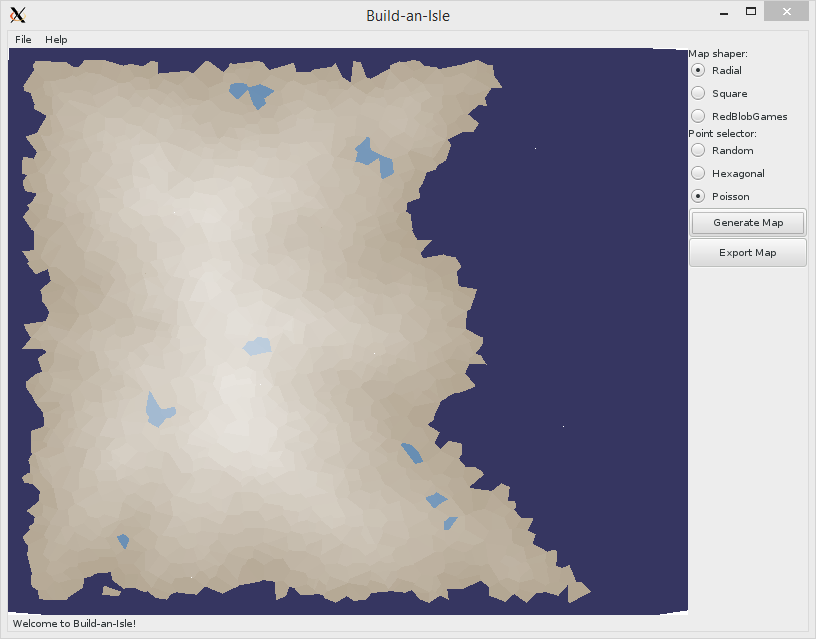
\includegraphics[width=0.7\linewidth]{poisson}
	\end{frame}

	\begin{frame}{Square}
		\centering
		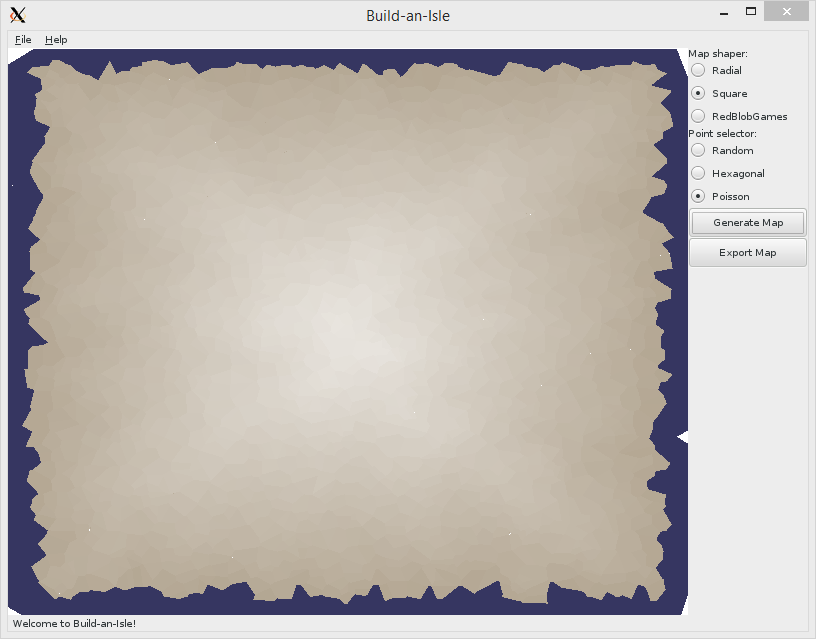
\includegraphics[width=0.7\linewidth]{square}
	\end{frame}

	\begin{frame}{Blob}
		\centering
		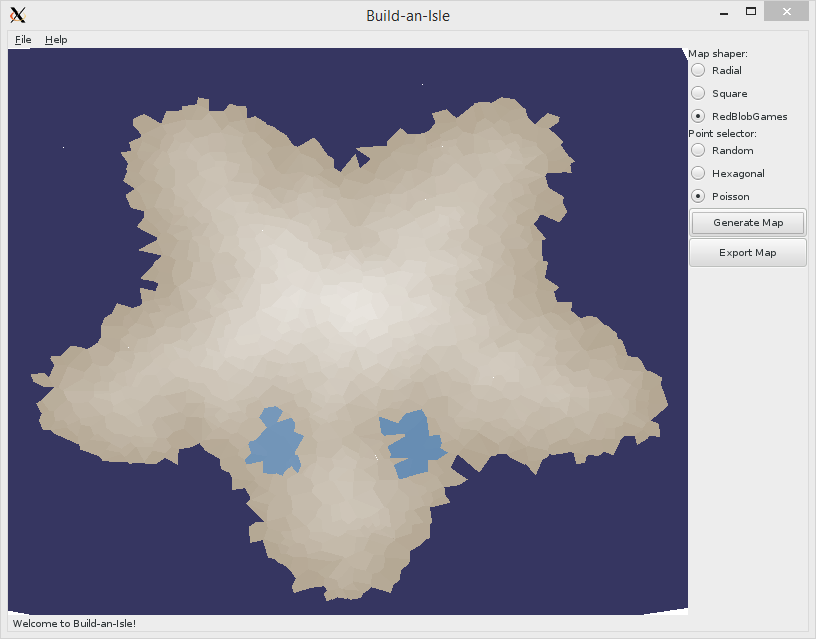
\includegraphics[width=0.7\linewidth]{blob}
	\end{frame}

	\section{Next steps}
	\begin{frame}{Next steps}
		\begin{itemize}
			\item Rivers
			\item Roads
			\item Threaded generation
			\item Realtime feedback
			\item Interactive viewer
		\end{itemize}
	\end{frame}

	\begin{frame}{}
	\end{frame}
\end{document}
